\hypertarget{results}{%
\section{Results}\label{results}}

\hypertarget{the-ground-state}{%
\subsection{The Ground State}\label{the-ground-state}}

\begin{figure}
\hypertarget{fig:fermion_gap_vs_L}{%
\centering
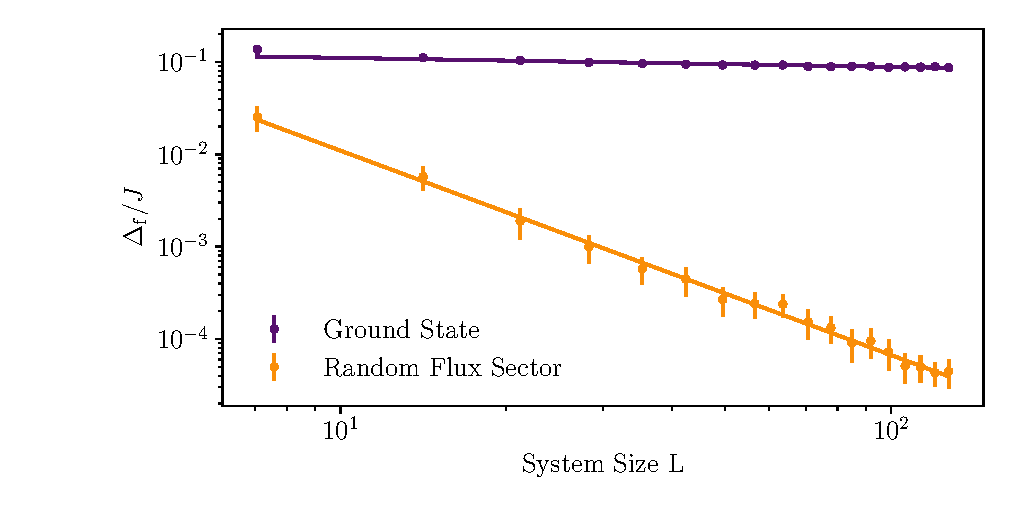
\includegraphics{figure_code/amk_chapter/results/fermion_gap_vs_L/fermion_gap_vs_L.pdf}
\caption{Within a flux sector, the fermion gap \(\Delta_f\) measures the
energy between the fermionic ground state and the first excited state.
This graph shows the fermion gap as a function of system size for the
ground state flux sector and for a configuration of random fluxes. We
see that the disorder induced by an putting the Kitaev model on an
amorphous lattice does not close the gap in the ground state. The gap
closes in the flux disordered limit is good evidence that the system
transitions to a gapless thermal metal state at high temperature. Each
point shows an average over 100 lattice realisations. System size \(L\)
is defined \(\sqrt{N}\) where N is the number of plaquettes in the
system. Error bars shown are \(3\) times the standard error of the mean.
The lines shown are fits of \(\tfrac{\Delta_f}{J} = aL ^ b\) with fit
parameters: Ground State: \(a = 0.138 \pm 0.002, b = -0.0972 \pm 0.004\)
Random Flux Sector:
\(a = 1.8 \pm 0.2, b = -2.21 \pm 0.03\)}\label{fig:fermion_gap_vs_L}
}
\end{figure}

\hypertarget{ground-state-phase-diagram}{%
\subsection{Ground State Phase
Diagram}\label{ground-state-phase-diagram}}

\hypertarget{the-flux-gap}{%
\subsection{The Flux Gap}\label{the-flux-gap}}

\hypertarget{conclusion}{%
\section{Conclusion}\label{conclusion}}

\hypertarget{discussion}{%
\subsection{Discussion}\label{discussion}}

\hypertarget{future-work}{%
\subsection{Future Work}\label{future-work}}

The Kitaev Honeycomb can be quite easily turned into a quantum error
correcting code \href{https://errorcorrectionzoo.org/c/honeycomb}{like
this}, the same idea applies to our model.

\begin{Shaded}
\begin{Highlighting}[]

\end{Highlighting}
\end{Shaded}
